%%%%%%%%%%%%%%%%%%%%%%%%%%%%%%%%%%%%%%%%%%%%%%%%%%%%%%%%%%%%%%%%%%
%%%%%%%% ICML 2014 EXAMPLE LATEX SUBMISSION FILE %%%%%%%%%%%%%%%%%
%%%%%%%%%%%%%%%%%%%%%%%%%%%%%%%%%%%%%%%%%%%%%%%%%%%%%%%%%%%%%%%%%%

% Use the following line _only_ if you're still using LaTeX 2.09.
%\documentstyle[icml2014,epsf,natbib]{article}
% If you rely on Latex2e packages, like most moden people use this:
\documentclass{article}

% use Times
\usepackage{times}
% For figures
\usepackage{graphicx} % more modern
%\usepackage{epsfig} % less modern
\usepackage{subfigure} 

% For citations
\usepackage{natbib}

% For algorithms
\usepackage{algorithm}
\usepackage{algorithmic}

% For graphics 
\usepackage{graphicx}

% As of 2011, we use the hyperref package to produce hyperlinks in the
% resulting PDF.  If this breaks your system, please commend out the
% following usepackage line and replace \usepackage{icml2014} with
% \usepackage[nohyperref]{icml2014} above.
\usepackage{hyperref}

% Packages hyperref and algorithmic misbehave sometimes.  We can fix
% this with the following command.
\newcommand{\theHalgorithm}{\arabic{algorithm}}

% Employ the following version of the ``usepackage'' statement for
% submitting the draft version of the paper for review.  This will set
% the note in the first column to ``Under review.  Do not distribute.''
\usepackage[accepted]{icml2014} 


% The \icmltitle you define below is probably too long as a header.
% Therefore, a short form for the running title is supplied here:
\icmltitlerunning{Kan,Sundhar,Yang,Sankar,Oliva}

\begin{document} 

\twocolumn[
\icmltitle{An ML Approach to Tala Classification\\COMP 562}

% It is OKAY to include author information, even for blind
% submissions: the style file will automatically remove it for you
% unless you've provided the [accepted] option to the icml2014
% package.
\icmlauthor{Alex Kan}{akan@unc.edu}
\icmlauthor{Akshay Sankar}{akshays@live.unc.edu }
\icmlauthor{Svetak Sundhar}{svetaksundhar@unc.edu}
\icmlauthor{Anthony Yang}{chunyang@live.unc.edu}
\icmlauthor{Dr. Junier Oliva}{joliva@cs.unc.edu}


% You may provide any keywords that you 
% find helpful for describing your paper; these are used to populate 
% the "keywords" metadata in the PDF but will not be shown in the document
\icmlkeywords{boring formatting information, machine learning}

\vskip 0.3in
]

\begin{abstract} 
	Carnatic Music is a sacred art form hailing from South India in the 18th century. This form of music has two main aspects: swara, or the melody and laya?, or rhythm. In this report, we investigate how we can classify the laya aspect, from audio samples of Carnatic Music. Specifically, we seek to identify the tala, or meter of the sample. This could potentially help discern the tala of a song for students of Carnatic Music, as Carnatic Music teachers are becoming harder and harder to find. We use the Carnatic Music dataset from the University of Pompeau Fabra. We attempt to use the 1D CNN, 2D CNN, RNN with Long Short term memory cells, and the Autoencoder (for denoising). This report provides our baseline results as well as the directions we plan to take this project.
\end{abstract} 
\section{Preprocessing Pipeline}

\subsection{State of the Art}
Currently, machine learning has been applied to Carnatic Music for Raga identification. That is, Kumar et. Al seeks to use SVM kernels to identify the scale of a certain audio sample. Currently, we are not aware of any literature that has been published to identify the meter of a given piece. To get started, we browsed through Google Brain\'s Magenta project. We observed that a lot of their publications were centered around generative music. We concluded that for the purposes of the COMP 562 class, we would stick to tala classification, but later plan on extending this paper into one where we generate Carnatic Music.
\subsection{Pipeline}
In order to preprocess our data, we extracted the song names and the corresponding meters, both of which were given in the dataset. After this, the song meters were encoded to integers for classification. After this, the dataset was made into a list of tuples. We then created random melspectrogram shots of about 3 seconds each. These were taken somewhere in between the 10th and the 80th seconds of the song. Each tuple consisted of the song name, the melspectrogram array, and the meter encoding.
	Then, a train and test split were created. This ratio was 80:20 respectively. After this, the key step of our preprocessing was performed. This was the reshaping of our features. We reshaped the size to 128x128x1 to pass it into our Convolutional Neural Network.


\section{Modeling} 

\subsection{Signal Processing Background}
	The primary unit of analysis for our process is the spectrogram. A spectrogram is a way of representing the frequencies of a given sound over time in a visual manner. A common way of representing a spectrogram is by using the mel scale rather than the Hertz scale; the mel scale allows us to measure the pitches of a sound as heard by listeners an equal distance from another. This is part of the key functionality of the librosa package, which we used extensively to load, featurize, and visualize our data. 
	Our CNN models were run on melspectrograms, and we eventually plan to run out Recurrent Neural Network model on melspectrograms with isolated Harmonic and Percussive components. We also stretched out our signals in terms of both time and pitch in order to determine how this would affect the accuracy of our models. 

\begin{figure}[ht!]
\centering
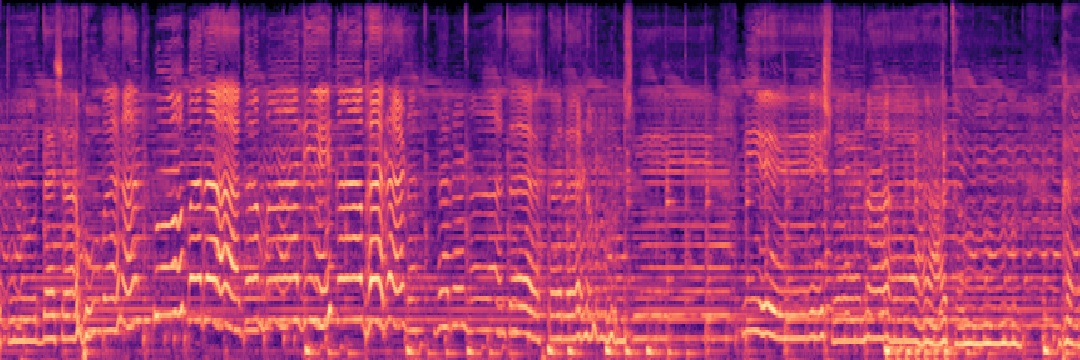
\includegraphics[width=82mm]{spectrogram.jpg}
\end{figure}

\subsection{Deep Learning}
 We reshaped our spectrograms such that they were 128x128, in order to decrease the number of features and speed up the training speed of our of model. Using the Keras library we used a Sequential model with seven layers. For our 3 hidden convolution layers, we used ReLU activation functions, followed by a Flatten layer with a dropout rate of 50 \%, a dense Layer with 64 nodes and a dropout rate of 50\%, and finally an output layer with a softmax activation function. 

We also used the Adam Optimzer to compile our model along with a Categorical Crossentropy function to evaluate our loss. 

 \subsection{Errors}
 The reason that our 1D and 2D ConvNet test accuracy was because of one common pitfall that we failed to avoid: the bleeding of data between our training and validation set. We trained on 5000 samples and validated and 925, but in our pipeline, there was a leak between the training and validation set. Thus, going forward, we will make sure that the training, validation, and test sets are all completely separated.
\subsection{Tables} 
 % Note use of \abovespace and \belowspace to get reasonable spacing 
% above and below tabular lines. 

\begin{table}[t]
\caption{Classification accuracies our models on the task of Tala prediction.}
\label{sample-table}
\vskip 0.15in
\begin{center}
\begin{small}
\begin{sc}
\begin{tabular}{lcccr}
\hline
\abovespace\belowspace
Model & Test Error \\
\hline
\abovespace
1D CNN    & 53\% \\
2D CNN & 92\%\\
RNN    & Still Running \\
\hline
\end{tabular}
\end{sc}
\end{small}
\end{center}
\vskip -0.1in
\end{table}
 
\subsection{Citations and References} 

1. Fu, S., Hu, T., Tsao, Y., \& Lu, X. (2017). Complex spectrogram enhancement by convolutional neural network with multi-metrics learning. 2017 IEEE 27th International Workshop on Machine Learning for Signal Processing (MLSP). doi:10.1109/mlsp.2017.8168119"

2. Kumar, V., Pandya, H., \& Jawahar, C. (2014). Identifying Ragas in Indian Music. 2014 22nd International Conference on Pattern Recognition. doi:10.1109/icpr.2014.142

3. Mcfee, B., Raffel, C., Liang, D., Ellis, D., Mcvicar, M., Battenberg, E., \& Nieto, O. (2015). Librosa: Audio and Music Signal Analysis in Python. Proceedings of the 14th Python in Science Conference. doi:10.25080/majora-7b98e3ed-003

4. Salamon, J., \& Bello, J. P. (2017). Deep Convolutional Neural Networks and Data Augmentation for Environmental Sound Classification. IEEE Signal Processing Letters, 24(3), 279-283. doi:10.1109/lsp.2017.2657381


\section*{Acknowledgments} 

We thank Dr. Junier Oliva for his guidance on our work thus far. He proposed that we do not use the Naive Bayes Model, and instead to try using RNNs. We have met with him once so far, but do plan to meet him again in the next couple of weeks.

\bibliography{example_paper}
\bibliographystyle{icml2014}

\end{document} 